\chapter{Results}\label{chap:Results}

A total of 15 participants from various disciplines including Natural Sciences, Social Sciences, Life Sciences and Computer Science evaluated Scholar Plot. We asked each participant to review the interface and then complete an online survey. Special care was taken to ensure that the participants had correct understanding about the visualization component before they began rating. The participants answered the questions on a Likert scale from 1 to 5 with 1 being strongly disagree and 5 being strongly agree.

Figure \ref{fig:UserStudy} illustrates the mean evaluation for each visualization component. Accuracy, Usability and understandability of Scholar Plot scored the highest $(\mu = 4.2)$ as it is very intuitive and can be used with minimal assistance. Many participants gave us feedback that they mostly liked the visual scheme of Scholar Plot. Another observation is that the participants agree to use Scholar Plot to evaluate themselves $(\mu = 4.1)$. They suggested that Scholar Plot can be improved by adding more funding agencies. Overall, this evaluation indicated that Scholar Plot is a user-friendly tool that complements the CV which can be used to review a scholar's accomplishments. The survey has been approved by the University of Houston Institutional Review Board (IRB).
 
 \begin{figure}[!htb]
  \centering
  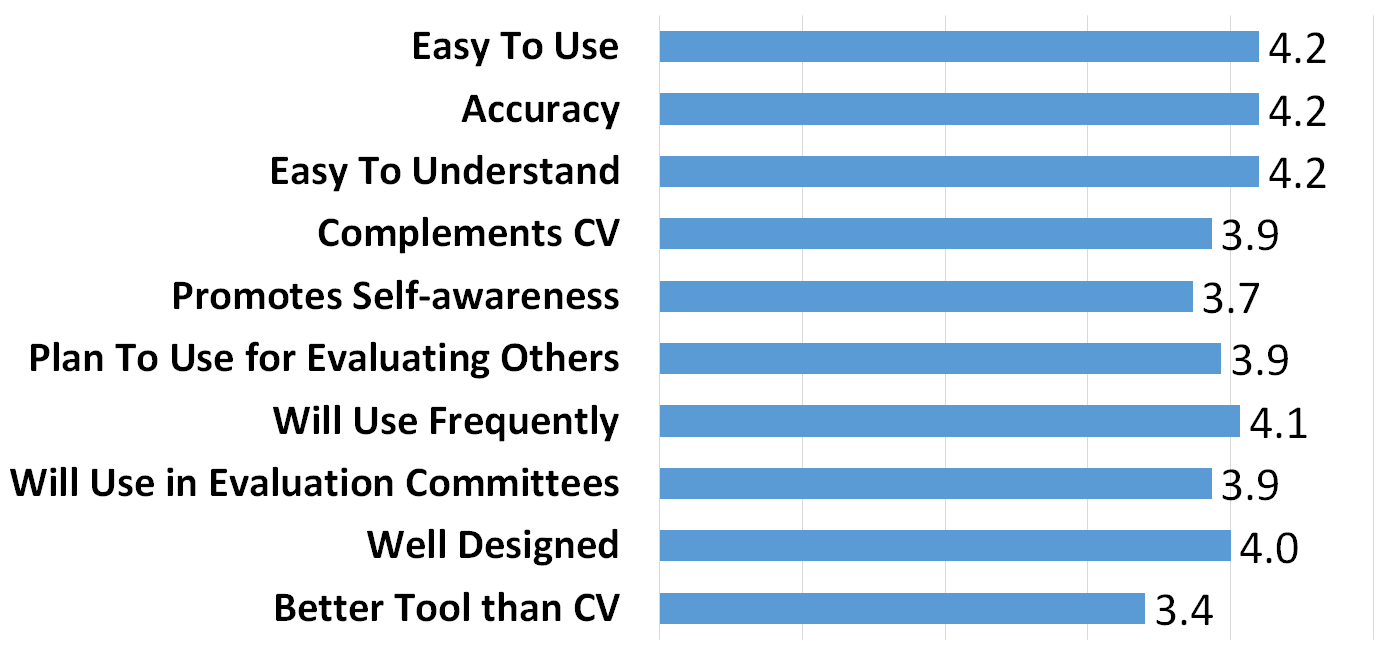
\includegraphics[width=\columnwidth]{figures/fig_survey_chart}
%  \vspace{-3ex} 
  \caption{Mean evaluation of Scholar Plot. A total of $n=15$ participants evaluated the survey.}
  \label{fig:UserStudy} 
\end{figure}